%\documentclass[conference,spanish,a4paper,10pt,oneside,final]{IEEEtran}
\nonstopmode
\documentclass[conference,spanish,a4paper,10pt,oneside,final]{tfmpd}

\include{conf/preconfig}
\include{conf/packages}
%
% Propiedades del documento: título, autor, etc
%
%% \newcommand{\titulo}{{\large FICH --- UNL}\\Procesamiento Digital de Imágenes
%% 2010\\Trabajo Final}
%% \newcommand{\autor}{Fornal, Esteban \and Pfarher, Christian \and Torrez, Mauro}
%% \newcommand{\fecha}{\today}
%% \newcommand{\tituloPDF}{Trabajo Final PDI 2010}
%% \newcommand{\autorPDF}{Fornal, Pfarher, Torrez}
%% \newcommand{\asuntoPDF}{}
%% \newcommand{\clavesPDF}{}
%
\include{conf/config}
%\include{conf/comandos}
%
\begin{document}
\title{Identificación de edificios y monumentos a partir de fotografías
tomadas con dispositivos móviles}
\author{Esteban C. Fornal, Christian N. Pfarher, Mauro J. Torrez\\
\textit{Trabajo práctico final de ``Procesamiento Digital de
Imágenes'', II-FICH-UNL.}}
\markboth{Procesamiento Digital de Imágenes: TRABAJO FINAL}{}
\maketitle
%
%
% %%%%%%%%%%%%%%%%%%%%%%%%%%%%%%%%%%%%%%%%%%%%%%%%%%%%%%%%%%%%%%%%%%%%%%%%%%%%%%
%
%
\begin{abstract}
%% El objetivo de este trabajo consiste en la identificación de edificios y
%% monumentos, a partir de imágenes obtenidas mediante un dispositivo móvil de
%% características estándar en el mercado. Para dicho propósito se plantearán
%% métodos diferentes, uno mediante extracción de características en el espacio
%% de la Transformada de Hough y otro basado en medidas estadísticas, comparando
%% a cada uno de ellos por separado y finalmente, evaluando el desempeño de la
%% utilización de ambos conjuntamente.
Se presenta un método para la identificación de edificios y monumentos, a
partir de fotografías tomadas con la cámara de un dispositivo móvil.
%Para la identificación 
Se extrae un vector de características \resalt{globales y locales?} de %la 
cada imagen.
%que es almacenado en una base de datos para su consulta.
Se presentan dos métodos para la extracción de características, %en la imagen
uno basado en la transformada de Hough y otro que utiliza estadísticas de los
histogramas. Se evalúa el desempeño utilizando \resalt{error cuadrático medio? para ambos...}
ambos métodos por separado y en
conjunto, para una base de datos de prueba de% unas pocas 
imágenes.
\end{abstract}
%
%
% %%%%%%%%%%%%%%%%%%%%%%%%%%%%%%%%%%%%%%%%%%%%%%%%%%%%%%%%%%%%%%%%%%%%%%%%%%%%%%
%
%
\begin{keywords}
Identificación%/reconocimiento 
de edificios, \eng{building recognition},
histograma, %extracción de características, 
transformada de Hough, clasificación.
\end{keywords}
%
%
% %%%%%%%%%%%%%%%%%%%%%%%%%%%%%%%%%%%%%%%%%%%%%%%%%%%%%%%%%%%%%%%%%%%%%%%%%%%%%%
%
%
\section{Introducción}
%README: esto es lo que estaba antes.. lo deje por las dudas porque al final me qued con la duda 
%si habia que corregirlo o no..
%por las dudas corrijo abajo y dejo  la version original...
%
%\PARstart{E}{n} la actualidad, la gran difusión de los dispositivos móviles nos
%permite llevar la información importante siempre con nosotros.
%Es muy común utilizar nuestros celulares, PDAs, además para \emph{obtener}
%información desde donde estamos, gracias a la proliferación de redes de datos
%inalámbricas.
%
%Dado que una gran parte de estos dispositivos además poseen una cámara
%digital, surge la idea de utilizarla junto con las conexiones de datos para
%obtener información acerca del lugar donde nos encontramos.
%
%Se presenta aquí una técnica de Procesamiento Digital de Imágenes orientada
%en este sentido, que permite la
%identificación de edificios, monumentos y otros puntos de interés, a partir
%de una fotografía capturada con un dispositivo móvil.
\PARstart{E}{n} la actualidad, la gran difusión de los dispositivos móviles nos
permite llevar la información importante siempre con nosotros.Además es muy 
común utilizar nuestros celulares, PDAs, GPS para \emph{obtener}
información desde cualquier lugar donde estemos, gracias a la proliferación de redes de datos
inalámbricas. Dado que una gran parte de estos dispositivos %además 
posee%n
una cámara
digital, surge la idea de utilizarla junto con las conexiones de datos para
obtener información acerca del lugar donde nos encontramos. Se presenta aquí %una 
un método que combina
técnicas de Procesamiento Digital de Imágenes orientadas
en este sentido, que permite la
identificación de edificios, monumentos y otros puntos de interés, a partir
de una fotografía capturada con un dispositivo móvil.
%
%
% %%%%%%%%%%%%%%%%%%%%%%%%%%%%%%%%%%%%%%%%%%%%%%%%%%%%%%%%%%%%%%%%%%%%%%%%%%%%%%
%
%
\section{Método propuesto}
En el método propuesto se ha puesto énfasis en la etapa de 
% que proponemos se basa en la 
extracción de características de la imagen, considerando
un método trivial de clasificación. % y la comparación de éstas con las de una base de datos.
%Esta 
La base de datos se generó tomando \resalt{$X$ ??} imágenes representativas 
de %l
cada monumento. %,
Se extrajeron sus características y se promediaron %promediándolas 
para obtener un prototipo ``generalizado'' de cada monumento/edificio 
% a detectar.
en particular.

\subsection*{Extracción de características}
\resalt{no se si es subsection* o subsection.. ver en la correción dice poner
subtitulo..}

La extracción de características se realiza en este trabajo mediante dos
técnicas diferentes:
\begin{enumerate}
\item %extracción de características 
por transformada de Hough, y
\item %extracción de características 
por estadísticas del histograma.
\end{enumerate}

%El entrenamiento de la base de datos se realiza obteniendo las características
%para cada imagen, junto a su etiqueta. %Para cada etiqueta, 
%Se extraen las características de todas las %las $X$ 
%imágenes %etiquetadas 
%con la misma etiqueta, y se guarda un
%``prototipo'' para esa clase, obtenido de promediar estas características.
%%, junto con la etiqueta.
%
%La clasificación de las imágenes consiste en % encontrar 
%obtener la etiqueta del prototipo, cuyas características 
%minimicen el error cuadrático medio con las de
%la imagen a identificar.

%% Lo de las 10+3 imágenes es parte de la prueba; lo de los prototipos
%% está arriba.....
%% Sobre diez de las trece imágenes de cada edificio, se aplicó el método de la
%% Transformada de Hough citado en este artículo, obteniéndose diez vectores
%% representativos (uno por cada imagen) y se procedió a promediar dichos vectores
%% dando como resultado un prototipo por cada edificio. De la misma manera se
%% realizó el mismo proceso, con el método estadístico descripto también en
%% este documento.
%
%%%%%%%%%%%%%%%%%%%%%%%%%%%%%%%%%%%%%%%%%%%%%%%%%%%%%%%%%%%%%%%%%%%%%%%%%%%%%%%%
%
\subsection*{Extracción de características mediante Transformada de Hough}
La transformada de Hough nos permite visualizar, a partir de una imagen de
bordes, los parámetros de aquellas rectas\footnote{El procedimiento es general,
sirve para cualquier geometría que se pueda expresar en términos de sus
parámetros. En este trabajo, se utiliza %os 
el espacio de los parámetros de las
rectas, el más sencillo.}
que son principales en la imagen.

Para la extracción de características con esta técnica se siguen los siguientes
pasos:
\begin{enumerate}
\item A partir de la imagen original, se obtiene %una 
su versión en escala de grises
      promediando los tres canales RGB, y se la escala a un tamaño normalizado.
\item Se obtiene una imagen de sólo bordes, aproximando la magnitud del
      gradiente según
      \begin{equation}
      \label{sob}
      \nabla f \approx |G_x| + |G_y|,
      \end{equation}
      donde $G_x$, $G_y$ son el resultado de aplicar los operadores gradiente
      de Sobel (fig. \ref{masksobel}) a la imagen. 
      Finalmente se umbraliza esta imagen de bordes %en 
      utilizando un parámetro $U$:
      \begin{equation}
      \label{umbral}
      f(x)=
      \begin{cases}
      0, & x\leq U\\
      255, & x > U
      \end{cases}
            \resalt{f(x,y) ? en realidad es f(intensidad) seria f(x,y) no?}
      \end{equation}

\item Con la imagen de bordes umbralizada se calcula la transformada de
      Hough para rectas.
\item Se aplica un escalado (submuestreo) a la transformada obtenida, llevándola
      a un tamaño
      pequeño %buscando 
      para obtener mayor tolerancia tanto en el parámetro angular
      $\theta$ como en el de distancia $\rho$.
\item Se toman los $N$ máximos de esta transformada y se guardan en el vector de
      características %las 
      sus coordenadas $(\rho,\theta)$, mapeadas al rango
      $[-1,1]$, obteniendo así un vector de $2N$ valores.
\end{enumerate}
El proceso completo puede verse en la Fig. \ref{procesohough}.
%% Como se puede observar en la Fig. \ref{procesohough}, en el primer paso se
%% obtiene una imagen de un solo canal mediante el promediado de los tres
%% canales RGB. Luego, con el objetivo de disminuir el costo computacional, se
%% realiza un redimensionamiento de la imagen de 640 x 480 pixels a 100x100.
%% Posteriormente, para la detección de bordes se aplica el operador gradiente
%% de sobel (\ref{sob}) y se umbraliza con la función definida en
%% (\ref{umbral}).
\begin{figure}
\begin{center}
\begin{tabular}{|c|c|c|}
\hline -1 & -2 & -1 \\\hline 0 & 0 & 0 \\\hline 1 & 2 & 1 \\\hline
\end{tabular}
\begin{tabular}{|c|c|c|}
\hline -1 & 0 & 1 \\\hline -2 & 0 & 2 \\\hline -1 & 0 & 1 \\\hline
\end{tabular}
\end{center}
\caption{Máscaras de filtrado (operadores gradiente) de Sobel.}
\label{masksobel}
\end{figure}
%% Tras estos pasos, se transforma al espacio de Hough y aquí se aplica
%% nuevamente un redimensionado a tamaño de 40x40 con el fin de tener una
%% tolerancia respecto a $\rho$ y $\theta$ del espacio transformado de Hough.
%% Finalmente, se obtienen las coordenadas $\rho$ y $\theta$ de 50 máximos con
%% las cuales se forma el vector de características representativo de la imagen.
\begin{figure}
\begin{center}
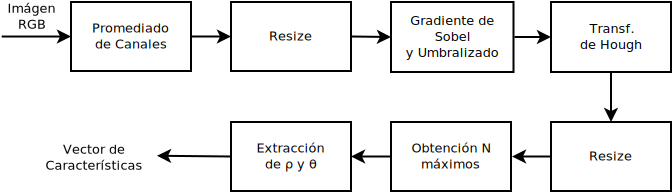
\includegraphics[scale=0.25]{../diagramas/procesohough} 
\end{center}
\caption{Proceso de extracción de características %la imagen mediante el método 
por %T. 
Transformada de Hough}
\label{procesohough}
\end{figure}
%
%%%%%%%%%%%%%%%%%%%%%%%%%%%%%%%%%%%%%%%%%%%%%%%%%%%%%%%%%%%%%%%%%%%%%%%%%%%%%%%%
%
\subsection*{Extracción de características por estadísticas del histograma}
A partir de la imagen original, se normaliza su tamaño y se toman 2 ``perfiles
de intensidad'' \resalt{promedio o acumulado?}: uno horizontal, calculado 
promediando\resalt{promediando?} cada columna de la
imagen, y otro vertical obtenido al promediar cada fila. También Se obtiene un
histograma de la imagen entera. De estos 3 vectores, se calculan
%y uno para cada perfil, 
y se guardan en el
vector de características la media aritmética $m$, la mediana $M$ (posición del
percentil 50),  y la desviación absoluta $D_{\T{abs}}$ respecto de la mediana:
\begin{equation*}
D_{\T{abs}}=\sum_i |x_i - M|
\end{equation*}
Así, se ha obtenido un vector de 9 valores que caracterizan% histogramas de la
a la imagen entera.

Con la idea de incorporar características locales, %Luego 
se subdivide \resalt{o subdividió -no se entiende la corrección} la imagen en cuatro 
cuadrantes y se obtienen, para cada uno, las mismas medidas que se calcularon para 
la imagen entera. Como resultado, se obtiene un vector de 45 características %a partir de
%histogramas que se
%guardarán en la base de datos para comparación.
asociado a cada imagen.

\begin{figure}
\begin{center}
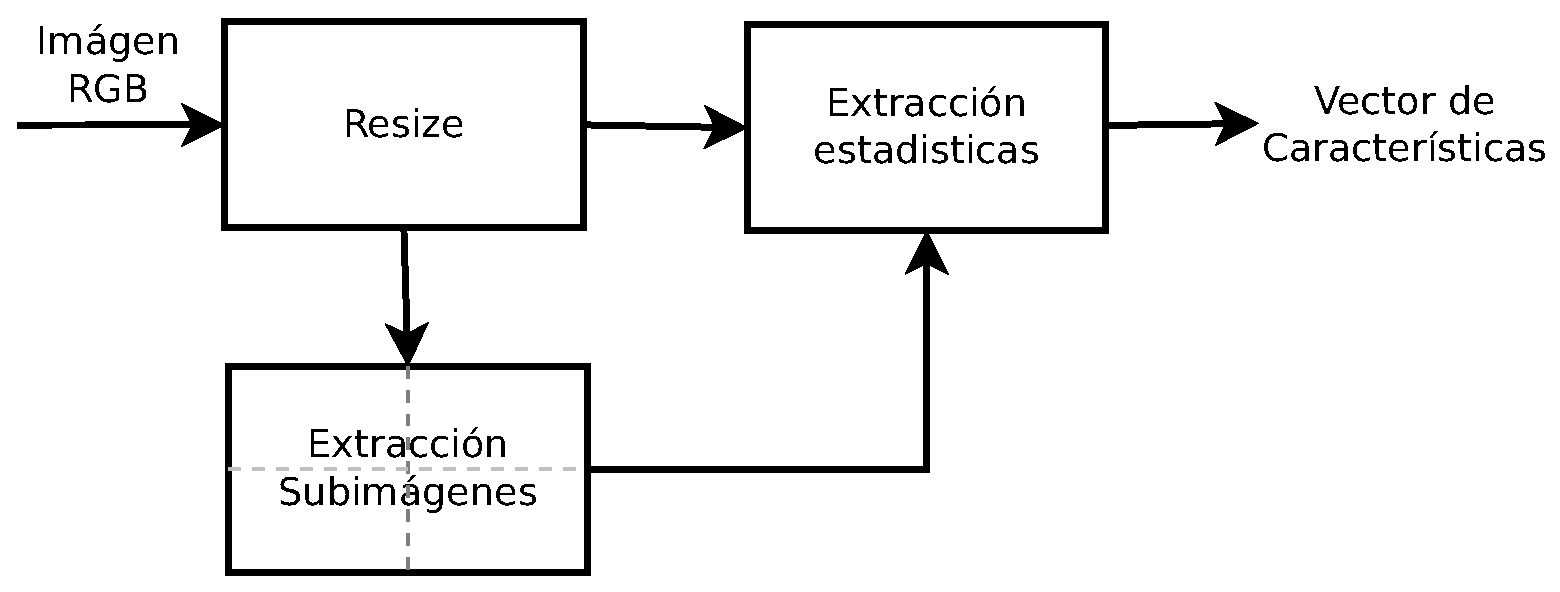
\includegraphics[scale=0.25]{../diagramas/procesoestadisticas} 
\end{center}
\caption{Proceso de extracción de características utilizando estadísticas del histograma}
\label{procesoestadisticas}
\end{figure}

\subsection{Clasificación}
\resalt{revisar si es subsecion* o subsection}
El entrenamiento de la base de datos se realiza obteniendo las características
para cada imagen, junto a su etiqueta. %Para cada etiqueta, 
Se extraen las características de todas las %las $X$ 
imágenes %etiquetadas 
con la misma etiqueta, y se guarda un
``prototipo'' para esa clase, obtenido de promediar estas características.
%, junto con la etiqueta.

La clasificación de las imágenes consiste en % encontrar 
obtener la etiqueta del prototipo, cuyas características 
minimicen el error cuadrático medio con las de
la imagen a identificar.
%
%
%%%%%%%%%%%%%%%%%%%%%%%%%%%%%%%%%%%%%%%%%%%%%%%%%%%%%%%%%%%%%%%%%%%%%%%%%%%%%%%%
%
%
\section{Base de datos}
\resalt{ver titulo de la sección..}
Las imágenes de prueba fueron tomadas con teléfonos celulares corrientes, a una
resolución VGA estándar de 640 píxeles de ancho por 480 de alto, en
diferentes condiciones
de iluminación: día a pleno sol, día nublado, noche, e interior, a monumentos/%
estatuas y edificios en diferentes lugares de la ciudad de Santa Fe (Argentina).
Se muestran en la figura \ref{imágenes} dos ejemplos de las mismas.
%
%
%%%%%%%%%%%%%%%%%%%%%%%%%%%%%%%%%%%%%%%%%%%%%%%%%%%%%%%%%%%%%%%%%%%%%%%%%%%%%%%%
%
%
\section{Experimentos y resultados}
%
%%%%%%%%%%%%%%%%%%%%%%%%%%%%%%%%%%%%%%%%%%%%%%%%%%%%%%%%%%%%%%%%%%%%%%%%%%%%%%%%
%
%\subsection{Descripción de las pruebas}
\subsection{Experimentación}
Para analizar %la prueba d
el método se utilizó validación cruzada, entrenando la base de
datos con 10 imágenes por clase y dejando 3 de prueba por cada clase.
\resalt{Se utilizaron
3 conjuntos de imágenes diferentes, con 5 clases cada uno.
Los conjuntos se formaron sorteando las 15 clases de imágenes disponibles en
3 de 5 clases cada uno. - Marcelo: no queda claro! Explicar simple:¨utilizaron N clases diferentes y se formaron 3 grupos
tomando 5 clases por cada uno aleatoria¨}

\begin{figure}
\begin{center}
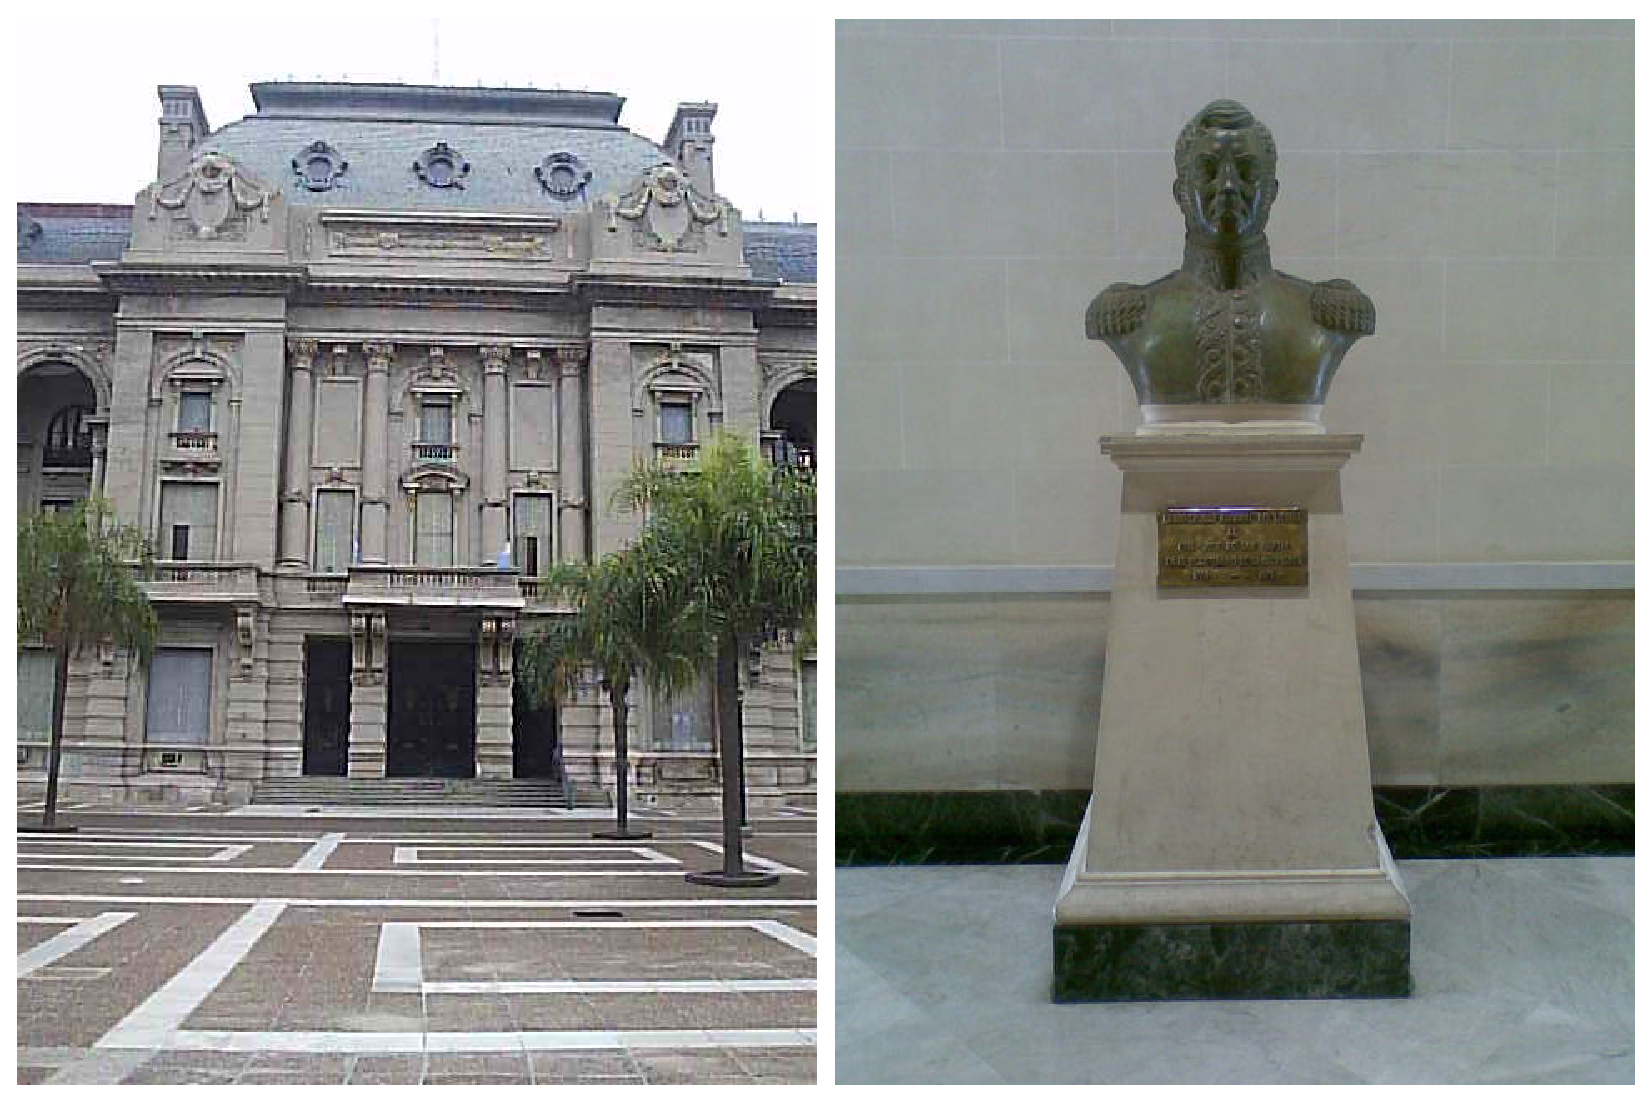
\includegraphics[scale=0.25]{../diagramas/dibujo} 
\end{center}
\caption{Ejemplo de dos imágenes utilizadas para probar el método.}
\label{imagenes}
\end{figure}

Se 
% probaron, en primer lugar, la 
clasificó utilizando extracción de características mediante
transformada de Hough y mediante histogramas por separado. Para el método de Hough
se probaron diferentes valores de $U$ (el umbral
aplicado a la imagen de bordes) y $N$ (el número de máximos en el espacio de
la transformada de Hough considerado). Mientras que, 
%a tener en cuenta para armar el vector de $2N$ características.
para el método de histograma se consideró el histograma y los perfiles del canal de
intensidad en el espacio de colores HSI.

Luego se evaluó el rendimiento del método utilizando todas las características %ambas técnicas 
en forma conjunta, para los parámetros de Hough $U$ y $N$ óptimos encontrados.

Se realizó además una prueba para las 15 clases de imágenes %en
del conjunto,
con el objetivo de tener una estimación de cómo responde %escala 
el método para un mayor número de imágenes.

Se considera la tasa de error ($\%$) del método según:
\begin{equation}
E_\%=100\cdot\frac{\T{número de errores}}{\T{número de pruebas}},
\end{equation}
considerando como error a cada prueba en que la imagen es mal etiquetada.

Cabe destacar que no se considera %como 
¨error¨ %la vez que 
cuando el método identifica
una imagen como el monumento acertado, pero en otras
condiciones de iluminación (cuando por ejemplo, la imagen de un monumento
tomada de día es clasificada como la del mismo monumento, pero tomada de noche).
Esta consideración se hace debido a que la detección de bordes elimina la
información de iluminación de la imagen; y está claro que no influye
en la clasificación por histograma; ya que éste varía significativamente
entre las versiones de día y noche, en particular, la media y mediana tendrán
valores bastante menores en la imagen nocturna que en aquella tomada de día.
Esto es además consistente con el objetivo del método, que es la correcta
identificación independientemente de las condiciones en que se toma la imagen.
%
% %%%%%%%%%%%%%%%%%%%%%%%%%%%%%%%%%%%%%%%%%%%%%%%%%%%%%%%%%%%%%%%%%%%%%%%%%%%%%%
%
\subsection{Resultados}

Los resultados de las pruebas con el método de Hough se muestran en la figura
\ref{graficaerror}. Se ha tomado un rango de valores representativos de $U$
y $N$ basados en pruebas previas, donde hemos identificado regiones de mínimo
error para $U~\in(60,120)$ y $N~\in(20,60)$.
En la misma figura, se puede apreciar que la tasa de error mínima se obtuvo
para un umbral $U = 100$ y unos $N = 30$ máximos (en promedio).

\begin{figure}
\begin{center}
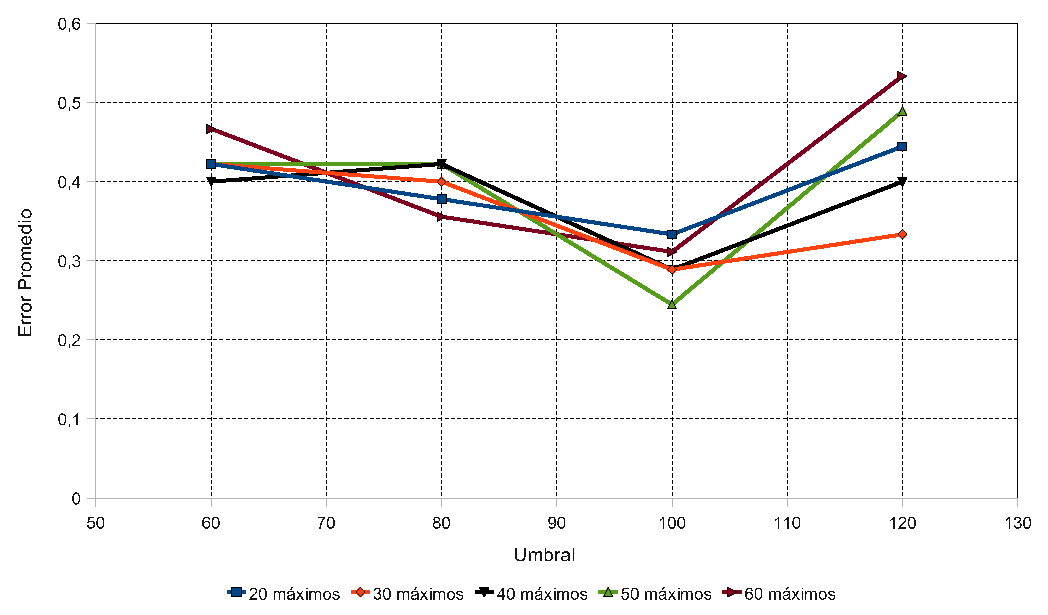
\includegraphics[width=8.5cm]{../diagramas/estadistica_noche_iguales} 
\end{center}
\caption{Error de clasificación promedio en función de distintos $U$ y $N$ para
el método de Hough.}
\label{graficaerror}
\end{figure}

%
%Debemos comentar aquí que para el método de Hough se realizaron una serie de pruebas
%que determinaron el rango representativo a analizar (umbral $U$ entre 60 y 120 y cantidad
%de máximos $N$ entre 20 y 60). 

En la tabla \ref{tablaerrores} se presentan los resultados para las pruebas
%iniciales 
con conjuntos de 5 clases%, y la estimación d
el resultado con
15 clases. 
%
%Cabe aclarar que en el primer caso se tomó un promedio de los errores
%sobre el conjunto.
%
\begin{table}
\caption{Tasas de error para los métodos}
\begin{center}\begin{tabular}{ccc}
\hline \emph{Método} & \emph{5 clases} & \emph{15 clases}\\ 
\hline Histogramas & 0\% & 0\%\\ 
\hline Hough & 35.5\% & 60.43\%\\ 
\hline Ambos & 2.22\% & 4.17\%\\ 
\hline 
\end{tabular}\end{center}
\label{tablaerrores}
\end{table}
%
Se puede observar que para el método de histogramas, la tasa de error fue cero
en ambas pruebas. En tanto que para el método de Hough, se obtiene menor tasa de
error con el conjunto de 5 clases que con el de 15, de 35.5\% y 60.43\%
respectivamente. En la última fila, se muestran los resultados de considerar todas
las características en conjunto, asignándole un peso equivalente a cada una. 

%
% %%%%%%%%%%%%%%%%%%%%%%%%%%%%%%%%%%%%%%%%%%%%%%%%%%%%%%%%%%%%%%%%%%%%%%%%%%%%%%
%
\subsection{Discusión}
A pesar de la muy buena performance del método de histograma, debemos tener
presente que los conjuntos de imágenes de entrenamiento/prueba para el método, 
han sido obtenidas en todos los casos a partir de una secuencia tomada en el 
lapso de unos minutos, lo cual implica que las condiciones de iluminación en
cada conjunto son prácticamente iguales. /resalt{aclarar antes lode los conjuntos sino aca no se entiende}
Los histogramas, miden la distribución estadística de los diferentes niveles
de intensidad presentes en la imagen, luego están estrechamente relacionados
con las condiciones de iluminación de la escena. Por este motivo, tenemos
que los histogramas entre las imágenes de entrenamiento/prueba son, a los
efectos prácticos, similares, lo cual explica el buen funcionamiento de este
método.

Se ha probado la técnica de histogramas sobre el canal I del espacio de color
HSI; por lo antes expuesto, debemos tener en cuenta consideraciones similares
para el resto de los canales de la imagen.

En general, se deberá poner énfasis en definir técnicas
de ``normalización'' orientadas a mejorar los resultados en condiciones más
realistas. Se deberá considerar la utilización de métodos de histograma
mejorados, por ejemplo el \emph{histograma de combinación espacial de DCT
ponderada} \cite{wdctsch}, \emph{vectores de coherencia de
color} \cite{Pass96histogramrefinement}, o el procesamiento de
histogramas borrosos presentado en \cite{Konstantinidis2005375}.

Respecto de la extracción de características mediante la transformada de Hough,
vemos que el rendimiento no es tan bueno como en la técnica de histogramas,
sin embargo en varios casos ha sido capaz de identificar correctamente edificios
a pesar de las diferentes condiciones de iluminación (día y noche), lo cual
es un resultado alentador.

No se puede evitar la mención al costo computacional del proceso, que aunque
no es tan elevado como para considerar impráctico el método, sí será una
limitante al considerar implementaciones en tiempo real o de alta velocidad
de respuesta: en una computadora promedio el cálculo se realiza en 1-2 segundos,
luego es esperable que este tiempo se triplique en un dispositivo móvil.

Se deberá considerar la utilización de un mejor detector de bordes, como el
propuesto por Canny \cite{canny}%\resalt{que tiene de bueno el de canny?}
, así como también técnicas de pre-procesamiento de la
imagen, como puede ser el filtrado homomórfico, en pos de mejorar los
resultados obtenidos en nuestras pruebas.

En lo que respecta a la escalabilidad de la base de datos, los resultados no
son particularmente alentadores, lo que nos obliga a considerar otra vez la
utilización de métodos más refinados de histograma y transformada de Hough.\resalt{esto no lo entiende marcelo}
%
%
% %%%%%%%%%%%%%%%%%%%%%%%%%%%%%%%%%%%%%%%%%%%%%%%%%%%%%%%%%%%%%%%%%%%%%%%%%%%%%%
%
%
\section{Conclusiones}
Se ha presentado una técnica para la identificación de edificios, monumentos,
esculturas con extracción de características mediante medidas de histograma
y transformada de Hough.

El rendimiento ha sido satisfactorio considerando las restricciones a las
que se han sometido las pruebas.

Se debe optimizar la implementación para portarlo a dispositivos móviles
con capacidad de procesamiento limitada.

Se hace necesario un preprocesamiento de la imagen, así como la incorporación
de métodos más refinados de extracción de características, para mejorar los
resultados obtenidos y así poder usar el método con una base de datos de
mayor magnitud.
%
%
% %%%%%%%%%%%%%%%%%%%%%%%%%%%%%%%%%%%%%%%%%%%%%%%%%%%%%%%%%%%%%%%%%%%%%%%%%%%%%%
%
%
\section{Trabajos futuros}
A partir del diseño aquí presentado, han surgido líneas para continuar investigando, 
y lograr un método más robusto:
%investigando esta técnica considerando las siguientes posibilidades:
\begin{itemize}
\item Aplicación de filtrado homomórfico y otros tipos de
      pre-procesamiento en las imágenes.
\item Aplicación de técnicas de \eng{warping} y otras transformaciones en busca
      de lograr invarianza respecto de rotación y escalado de la imagen.
\item Desarrollo de técnicas de extracción de características más robustas.
\item Desarrollo de una implementación óptima para dispositivos móviles con
      poder de procesamiento limitado.
\end{itemize}
\nocite{*}
\bibliographystyle{tfmpd}
\bibliography{tfmpd}
\end{document}
